
\section{Introduction}
\subsection{Outline}

\begin{frame}
  \frametitle{Review of Last Week}
  \begin{itemize}
  \item {\bf Search Algorithms} are defined by the systematic checking of the {\bf Search Space} of a problem;\bigskip

  \item We studied three types of Search Algorithms:
    \begin{itemize}
    \item Complete Search
    \item Divide and Conquer
    \item Greedy Search
    \end{itemize}
  \end{itemize}
  \bigskip

  \begin{block}{}
    This week we introduce a fourth search algorithm: {\bf Dynamic Programming}.
    \medskip

    Dynamic Programming is arguably the most used algorithm in programming competitions. It's basic idea is that we can exchange "computation time" for "memory".
  \end{block}
\end{frame}

\subsection{Intro to Dynamic Programming}
\begin{frame}
  \frametitle{What is Dynamic Programming (DP)?}

  \structure{DP} is a \structure{Search Algorithm} based on the idea of {\bf building partial solutions} and storing them on memory.

  \bigskip

  \begin{block}{Basic Idea of DP}
    \begin{itemize}
      \item Create a {\bf DP table} where the axis are the parameters of a recurrent function that generates the solution to the problem; \bigskip

      \item Fill in the table with the starting condition of the recurrence;\bigskip

      \item Fill in the rest of the table recursively or or using an iterator, and find the answer;
    \end{itemize}
  \end{block}
\end{frame}

\begin{frame}{What is Dynamic Programming (DP)?}{Characteristics}

  \begin{block}{When is DP useful?}
    In programming contests, a problem that requires \structure{optimization} or \structure{counting} "smells of DP"
    \begin{itemize}
    \item ``Count the number of solutions...''
    \item ``Find the minimum cost...''
    \item ``Find the maximum length...''
    \end{itemize}
  \end{block}

  \begin{exampleblock}{What is the running cost of DP?}
    The DP algorithm evaluates each element of the DP table.\medskip

    Therefore, DP costs "size of DP table $\times$ cost of one element.\medskip

  \end{exampleblock}
  The proof of correctness of DP algorithm is {\bf Proof by Induction}.
\end{frame}

\subsection{Example Problem}

\begin{frame}
    \frametitle{Problem Example: Wedding Shopping -- UVA 11450}

    \begin{block}{}
      Best way to understand DP is to \structure{do a lot of examples!}
    \end{block}

    \begin{columns}
      \column{0.7\textwidth}
    Problem summary:
    \begin{itemize}
      \item There are $C$ classes of items;
      \item Each class has $K_c$ options;
      \item Each option $K_{c,i}$ has a different cost;
      \bigskip

      \item Buy one of each option from each Class;
      \item Maximize the total cost;
      \item {\bf However}, you cannot exceed the budget $M$
      \bigskip

      \item $M \leq 200$, $1 < C \leq 20$, $0 < K_c \leq 20$
    \end{itemize}

      \column{0.3\textwidth}
      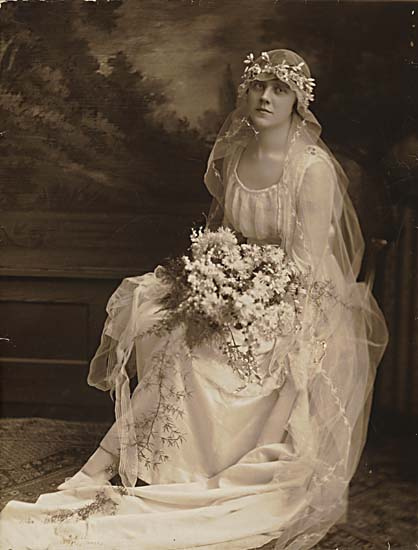
\includegraphics[width=.8\textwidth]{../img/weddingdress}\\
    \end{columns}\bigskip

    The total number of possible buying combinations is $20^{20}$

    \ppagenote{Wedding Dress Image CC-By-2.0 by \url{https://www.flickr.com/photos/vancouver125/5634967507}}
\end{frame}

\begin{frame}{Problem Example: Wedding Shopping -- UVA 11450}{Solution Example}
  \begin{block}{Sample case 1: $C=3, K_c = \{3,2,4\}$}
  \begin{tabular}{|c|cccc|}
    Class & 1 & 2 & 3 & 4\\
    \hline
    $K_0$ & 6 & 4 & 8 & \\
    $K_1$ & 5 & 10 & & \\
    $K_2$ & 1 & 5 & 3 & 5\\
  \end{tabular}
  \end{block}
  \medskip

  If budget $M=20$, the answer is \alert{19}. You can reach this answer by buying:
  \begin{itemize}
    \item $8(K_{0,2})+10(K_{1,1})+1(K_{2,0})$
    \item $6(K_{0,0})+10(K_{1,1})+3(K_{2,2})$
    \item $4(K_{0,1})+10(K_{1,1})+5(K_{2,1} \text{ or } K_{2,3})$
  \end{itemize}
  \bigskip

  However, if $M=9$, There is no solution for the problem, because the minimum possible cost is $10$, or $4(K_{0,1})+5(K_{1,0})+1(K_{2,0})$
\end{frame}

\begin{frame}[fragile]{Problem Example: Wedding Shopping -- UVA 11450}{Complete Search Solution}
  This is a {\bf Search problem}: our solution selects one item from each class. Unfortunately, the \emph{Greedy} approach does not work here.
  \begin{block}{Recursive Complete Search}
    \begin{itemize}
      \item Function \structure{shop$(m,g)$} finds the best item to buy in $K_g$ after spending $m$, and return the remaining budget;

      \item It tests every $K_{g,i}$ by first calling \structure{shop$(m+K_{g,i}, g+1)$}, recursively;

      \item End condition 1: $m > M$, return -1
      \item End condition 2: \structure{shop$(m,|C|)$}, return $m$
      \item The initial call: \structure{shop$(0,0)$}.
    \end{itemize}
  \end{block}
{\smaller
\begin{verbatim}
shop(m,g):
  if (m > M) return -1                           // no money
  if (g == C) return m                           // one solution
  return (max(shop(m+price[g][i], g+1)), i in Kc)// choose max
\end{verbatim}}


\end{frame}

\begin{frame}{Wedding Shopping (11450) - Complete search}{Time Limited Exceeded}
  The {\bf complete search} solution works, but because we have a total of $20^{20}$ possible choices, it does not finish in time;\bigskip

  \alert{Problem: Too many overlapping subproblems}


  \begin{block}{Sample case}
    \medskip
    \begin{columns}[T]
      \column{0.4\textwidth}
      \begin{tabular}{|c|cccc|}
        Class & 1 & 2 & 3 & 4\\
        \hline
        0 & 6 & 4 & 8 & 12\\
        1 & 4 & 6 & 6 & 2\\
        2 & 1 & 5 & 1 & 5\\
        3 & 2 & 4 & 6 & 2\\
      \end{tabular}
      \column{0.4\textwidth}
      How many times the program does the function calls \emph{shop(10,2)}?\bigskip

      Every time \emph{shop(10,2)} is called, the return value is always the same.
    \end{columns}
  \end{block}
  Is it possible to reduce the number of identical calls?
\end{frame}


\begin{frame}
  \frametitle{Wedding Shopping -- the DP approach}

  When a problem has this characteristic ({\bf repeated sub-structures}), it is a strong hint that DP is a good solution.
  \bigskip

  First, we create a {\bf DP table} using the parameters of the "shop" recurrent function.

  \begin{block}{How big is the table?}
    The table stores all possible calls of \emph{shop(m,g)}, so the table size is $|M| \times |C|$.
    \bigskip

    Remember that $0 \leq M \leq 200$ and $1 < C \leq 20$, so our table has \alert{$201*20=4020$ states}.
  \end{block}
  \smallskip

  That is a very small number! This algorithm will be FAST.
\end{frame}

\begin{frame}{Wedding Shopping -- the DP approach}{How to fill the table?}

  There are two main approaches for filling the {\bf DP table}:
  \bigskip

  \begin{itemize}
  \item {\bf Top-down approach}: \\Use the DP table as a look-up (memory) table. Every time you visit a state, save the result and do not recalculate. Very common with {\bf recursion}.
  \vfill

  \item \structure{Bottom-up approach}: \\ First complete the starting values of the table, then progressively fill the other states based on the starting ones. Very common with {\bf for loops}.
  \end{itemize}
\end{frame}

%%%%%%%%%%%%%%
%% Solution: Dynamic Programming
% Programming here is not "code", but a "tabular method" (table method)

%% DP us normally used when
% Program has optimal sub structure:
%   The optimal solution to the problem contain optimal solutions to sub problems
%   - "similar" to the requirement of greedy
%   - If you can make a complete search recurrent (recursive), then you have this
% The subproblems are overlapping
%   - The number of _Distinct_ subproblems is small, but they are computed repeatedly
%   - Different from divide and conquer, in DC the sub problems are distinct
%%%%%%%%%%%%%

\begin{frame}[fragile]{Wedding Shopping -- the DP approach}{Top-down DP}

\begin{block}{}
{\smaller
\begin{verbatim}
memset(table, -2, sizeof(table))            //-2 = "not visited"

shop(m,g):
  if (m > M) return -1                      // no money
  if (g == C) return m                      // one solution
  if (table[m][g] != -2) return table[m][g] // table lookup

  table[m][g] = (max(shop(m+price[g][i],[g+1])), i in Kc)
  return table[m,g]                         // calculate&return
\end{verbatim}}
\end{block}
\vfill

\begin{block}{Top Down DP Implementation is very easy}
  Just add a table, and every time you enter your recursive function, test if the parameters exist in the table.
\end{block}

\begin{alertblock}{}
  Make sure that the result of your function is {\bf always the same} when the DP parameters are the same! (usually not a problem)
\end{alertblock}
\end{frame}

%%% TODO: Add how to print after the bottom up DP
%% What if you need to print the result (maybe not add this?)
% for each level, you check the lower level to see which one matches the current state
% See slide 16 for details

\begin{frame}
  \frametitle{Wedding Shopping -- bottom-up DP}
  Algorithm:
  \begin{itemize}
  \item Prepare a table with the problem states (same as top-down);
  \item Add the the initial values in the table as "unprocessed";
  \item {\bf (Loop)} For each unprocessed value, process it, and add the new unprocessed values.
  \end{itemize}

  \vfill

  The main difficulty in bottom-up DP is to find the base cases and the transition function. After that, it is just a big for loop.
\end{frame}

\begin{frame}
  \frametitle{Wedding Shopping -- Bottom-up DP}

  Example: M=10, \alert<2>{$K_0=\{2,4\}$}, \alert<3>{$K_1=\{4,6\}$}, \alert<4>{$K_2=\{1,3,2,1\}$}
  \bigskip

  \begin{tabular}{|c||c|c|c|c|c|c|c|c|c|c|c|c|}
    \hline
    M & 0 & 1 & 2 & 3 & 4 & 5 & 6 & 7 & 8 & 9 & 10\\
    \hline
    $s=0$ & X & & & & & & & & & & \\
    $s=1$ & & & \only<2->{X} & & \only<2->{X} & & & & & & \\
    $s=2$ & & & & & & & \only<3->{X} & & \only<3->{X} & & \only<3->{X}\\
    $s=3$ & & & & & & & & \only<4->{X} & \only<4->{X} & \only<4->{X} & \only<4->{X}\\
    \hline
  \end{tabular}

  \begin{itemize}
  \item {\bf Start state}: We use no money, so mark $T(0,0)$
  \item {\bf Transition $(s \to s+1)$}:
    \begin{itemize}
      \item Loop: $i = 0 \to m$
      \item If $T(s,i)$ is marked:
      \begin{itemize}
        \item Loop: $j = 0\to |K_c|$
        \item Mark $T(s+1,i+K_{c,j})$
      \end{itemize}
    \end{itemize}
  \item {\bf Solution}: Maximum marked column of the last row.
  \item {\bf Note}: Other solutions are possible!
  \end{itemize}
\end{frame}

\begin{frame}[fragile]{Wedding Shopping -- Bottom-up DP}

  Example: M=10, \alert<2>{$K_0=\{2,4\}$}, \alert<3>{$K_1=\{4,6\}$}, \alert<4>{$K_2=\{1,3,2,1\}$}
  \bigskip

  \begin{tabular}{|c||c|c|c|c|c|c|c|c|c|c|c|c|}
    \hline
    M & 0 & 1 & 2 & 3 & 4 & 5 & 6 & 7 & 8 & 9 & 10\\
    \hline
    $s=0$ & X & & & & & & & & & & \\
    $s=1$ & & & X & & X & & & & & & \\
    $s=2$ & & & & & & & X & & X & & X\\
    $s=3$ & & & & & & & & X & X & X & X\\
    \hline
  \end{tabular}
  {\smaller
  \begin{block}{}
\begin{verbatim}
memset(table,0,sizeof(table))
table[0][0] = 1

for g in (0 to C-1)
  for i in (0 to M-1):
    if table[g][i] == 1:
       for k in (0 to K[g]-1):
          table[g + 1][i + cost[g][k]] = 1
            ## omitted out of bounds check!
\end{verbatim}
  \end{block}}
\end{frame}

\subsection{Considerations}

\begin{frame}
  \frametitle{DP: Top-down or Bottom-up?}

  \begin{block}{Top-Down}
    \structure{Pros:}\\
    Easy to implement, just add memory to a recursive search. Only computes the visited states of the DP table.

    \alert{Cons:}\\
    Overhead of recursive function (especially python!). Hard to reduce the size of the DP table.
  \end{block}

  \begin{block}{Bottom-Up}
    \structure{Pros:}\\
    Faster if you will visit the entire DP table anyway. It is possible to save memory by discarding old rows.

    \alert{Cons:}\\
    Can be harder to create the algorithm. If the DP table is sparse, the loop will visit every state.
  \end{block}
\end{frame}

\begin{frame}{Finding the Decision Set with DP}

  \begin{block}{}
    In the first example, the solution is only the final money. However, in other examples, you also need to know the {\bf decisions} used to reach that result.\bigskip

    {\bf Example}: Print the path with the smallest cost;
  \end{block}
  \bigskip

  It is not very hard to solve this problem. It just requires TWO tables:
  \begin{itemize}
    \item The DP table that we already know;
    \item The "Parent" table, which indicate which cell led to the current one;
  \end{itemize}
  \bigskip

  The next example will show the use of the "Parent" table.\bigskip

  Be careful how the problem break ties between identical solutions (lexographic order, first found, any order, etc.)
\end{frame}

\subsection{Pathfinding DP Example}
\begin{frame}{Example 2: Apple Field}
  \begin{block}{}
  {\smaller
  A farmer has an apple field, and a robot to collect the apples. However, the robot can only move {\bf left} and {\bf down}. The robot starts at position $(0,0)$, and ends at $(n,n)$.\medskip

  For each cell in the field, you know how many apples the robot can pick. Find the path that maximizes the number of apples the robot picks.
}
  \end{block}

  \begin{center}
    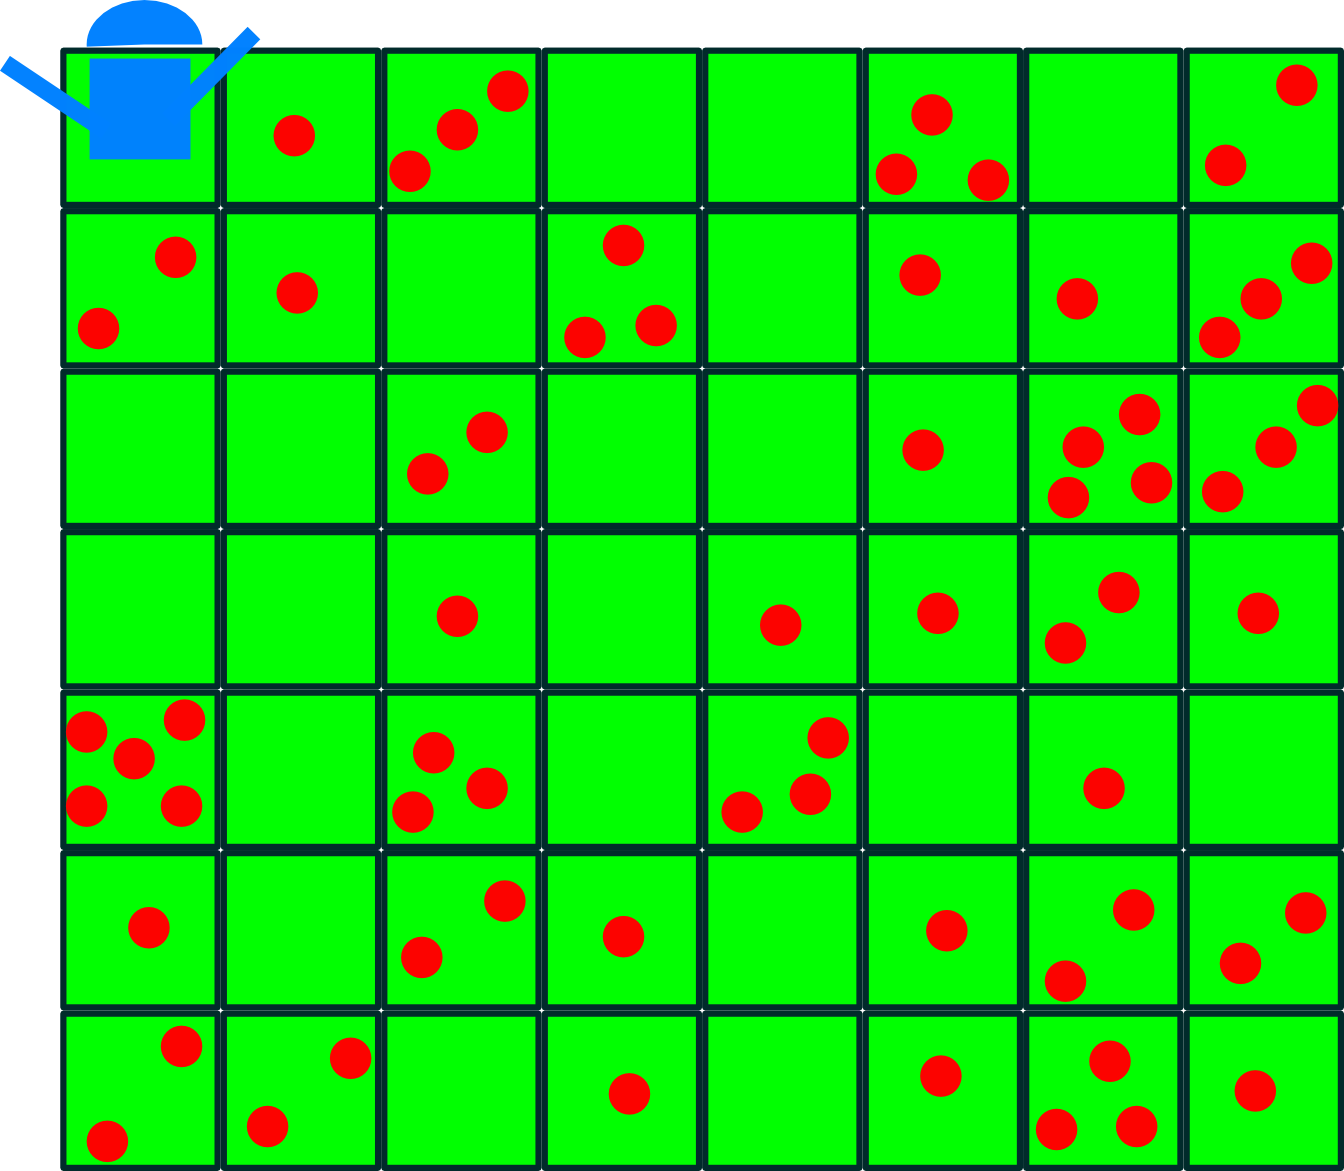
\includegraphics[width=0.5\textwidth]{../img/applefield}
  \end{center}
\end{frame}

\begin{frame}{Example 2: Apple Field}{Complete Search}

  \begin{center}
    {\smaller One possible solution (not-maximum)}\\
    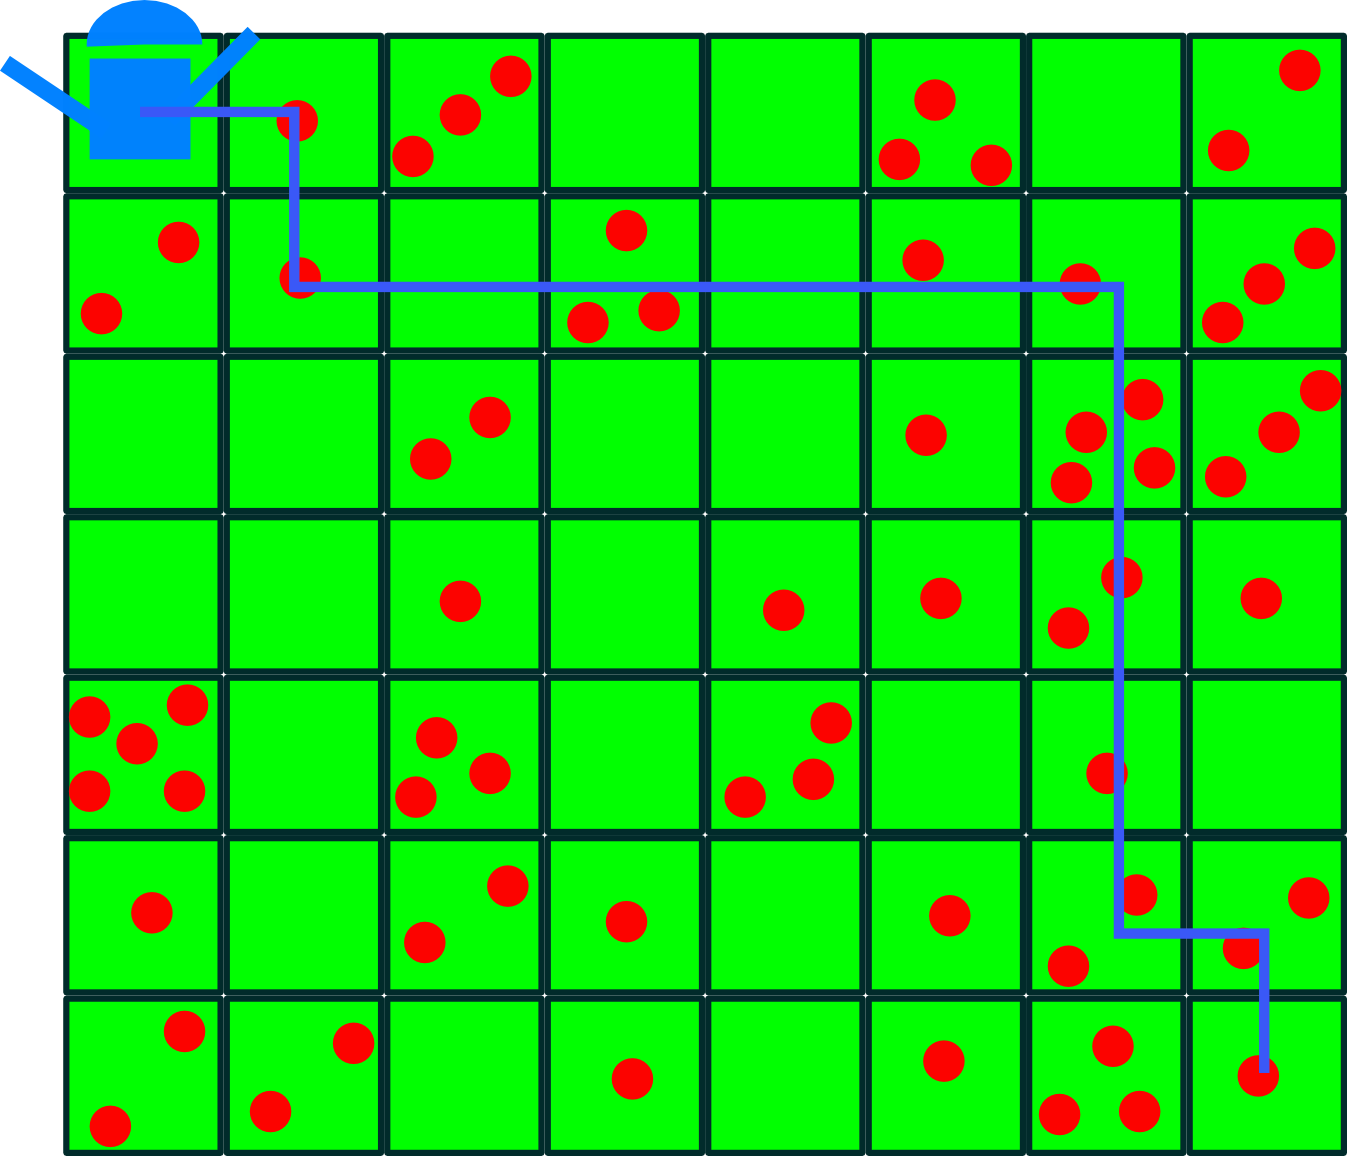
\includegraphics[width=0.5\textwidth]{../img/applefield-solution}
  \end{center}

  How many different paths are possible? Answer: $\binom{2n}{n} = \frac{(2n)!}{n!n!}$.
  \bigskip

  Is it necessary to check every path? Or overlapping states exist?
\end{frame}

\begin{frame}{Example 2: Apple Field}{Overlapping Solutions}
  \begin{center}
    {\smaller One possible (non-optimal) solution}\\
    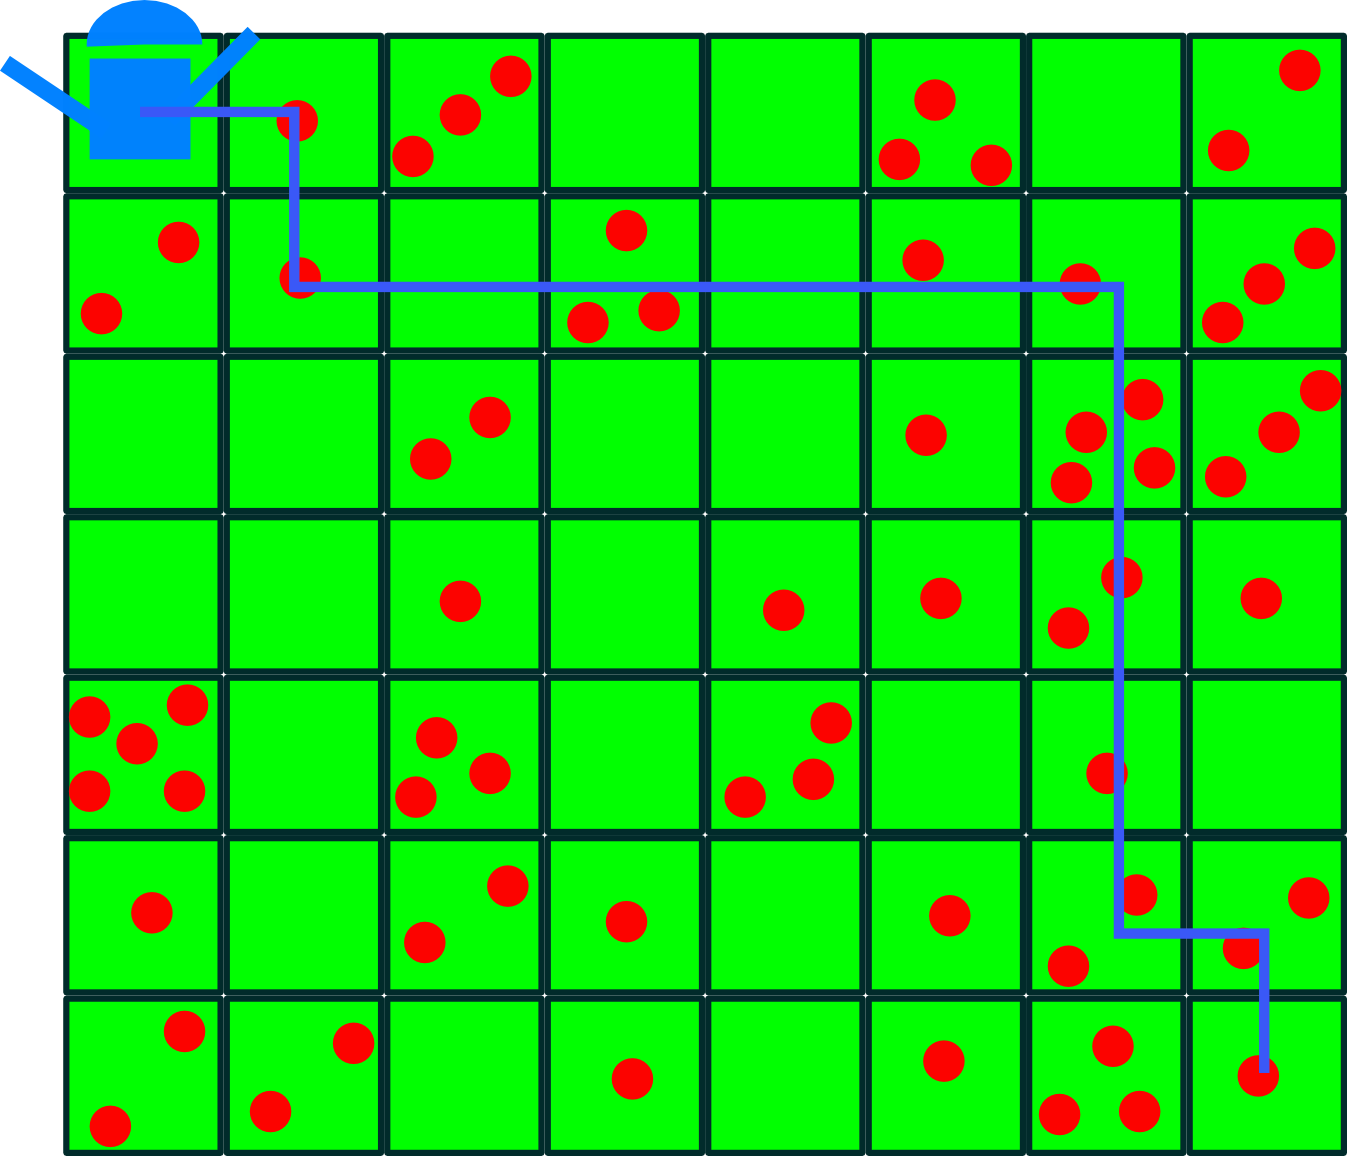
\includegraphics[width=0.5\textwidth]{../img/applefield-solution}
  \end{center}

  {\smaller
  For any $(x,y)$, the maximum path $(x,y) \to (n,n)$ does not depend on the path $(0,0) \to (x,y)$. This let us create a DP table based on the current position of the robot.}
\end{frame}

\begin{frame}{Example 2: Apple Field}{Bottom-up DP}
  \begin{itemize}
  \item {\bf DP table and Parent table:}
  \begin{itemize}
    \item The DP table is a $n+1\times n+1$ table. At every position, we have the maximum number of apples from $(0,0)\to(x,y)$.
    \item The Parent table is a $n+1\times n+1$ table. At every position, we store the last-1 cell (up or right) of $(0,0)\to(x,y)$.
  \end{itemize}

  \item {\bf Initial Condition:} (DP table only)
  \begin{itemize}
    \item To avoid special treatment of the first row and first column, we include a "boundary" at the top and right of the table. Every cell at the boundary has "0" apples
  \end{itemize}

  \item {\bf Transition:}
  \begin{itemize}
    \item We double loop over the DP table (row $\to$ column, or vice-versa). For every cell $(x,y)$:\\
    $DP[x][y] = \text{apple}[x][y] + \text{max}(DP[x-1][y],DP[x][y-1])$\\
    $\text{Parent}[x][y] = (DP[x-1][y] > DP[x][y-1]?\leftarrow:\uparrow)$
  \end{itemize}
  \end{itemize}
\end{frame}

\begin{frame}[fragile]{Example 2: Apple Field}{Pseudocode}
  {\smaller
  \begin{block}{}
\begin{verbatim}
int apple[m+1][n+1];
// Input Data. Requires some preprocessing:
//   - Valid data is put 1 to m, 1 to n.

int DP[m+1][n+1];        // Intialized to -1
DP[0][1] = 0;            // Initial state;
int parent[m+1][n+1][2]; // store (x,y) of parent

for (int i = 1; i < m+1; i++) {
  for (int j = 1; j < n+1; j++) {
    DP[m][n] = apple[m][n] + max(DP[m][n-1], DP[m-1][n]);
    if (DP[m][n-1] > DP[m-1][n]):
       parent[m][n][0] = m; parent[m][n][1] = n-1;
    else:
       parent[m][n][0] = m-1; parent[m][n][1] = n;
  }
}
\end{verbatim}
\end{block}
  }
\end{frame}

\begin{frame}{Example 2: Apple Field}{Simulating the algorithm}

\begin{columns}
  \column{0.5\textwidth}
  \begin{center}
    Input Table\\
    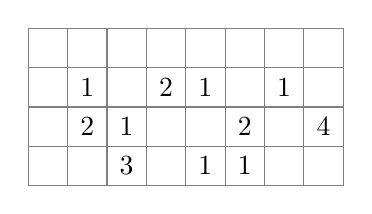
\begin{tikzpicture}
    \draw[step=0.5cm,color=gray] (0,0) grid (4,2);
    %% Row 1
    \node at (.75,1.25) {1};
    \node at (1.75,1.25) {2};
    \node at (2.25,1.25) {1};
    \node at (3.25,1.25) {1};
    %% Row 2
    \node at (.75,.75) {2};
    \node at (1.25,.75) {1};
    \node at (2.75,.75) {2};
    \node at (3.75,.75) {4};
    %% Row 3
    \node at (1.25,.25) {3};
    \node at (2.25,.25) {1};
    \node at (2.75,.25) {1};
    \end{tikzpicture}
  \end{center}

  \column{0.5\textwidth}
  \begin{center}
  DP Table\\
    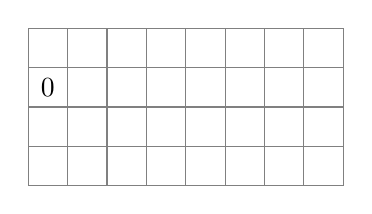
\begin{tikzpicture}
    \draw[step=0.5cm,color=gray] (0,0) grid (4,2);
    \node at (.25,1.25) {0};
    \end{tikzpicture}
  \end{center}
\end{columns}

\end{frame}

%\subsection{Flight Planner}
%%%%%%%%%%%%%
%% Example 2 -- UVA 10337 Flight Planner
% 1 Mile Altitude and 1(x100) miles distance
% wind speed map
% fuel cost: Climb +60, hold +30, sink +20 - windspeed wsp[alt][dis]
% Compute min fuel cost from (0,0) to (0,X=4)

%% First guess: Complete search/Backtracking finding path with minimal fuel cost
% Recurrence: minimum of current + climb/Hold/Dive
% Problem: 1000 distance columns: 3^1000 states to search!
% However, there are MANY overlapps: at any column/height, former path does not matter.

%% DP solution
% TOP down: create a 2D table and store computation value of subproblems as they are seen.
% Bottom-up: Start at 0 fuel used. Calculate next column based on where current column can reach
%            Bottom up hint: We just need to store two columns at a time (if only final result is desired)

\section{Classical DP}
\begin{frame}{Classical DP Problems}
  There are some categories of problems that are considered to be "classical DP problems".
  \bigskip

  \begin{itemize}
    \item Max sum;
    \item Max sum 2D;
    \item Longest Increasing Subsequence;
    \item Knapsack Problem;
    \item Coin Change;
  \end{itemize}
  \bigskip

  We will show some examples from each category so you can have a better understanding of the DP philosophy.\bigskip

  {\bf QUIZ}: For each problem, after the problem is explained please spend 10 minutes finding the {\bf DP table}, and the {\bf transition}.
\end{frame}

\subsection{Max Sum}

\begin{frame}[fragile]{The 1D Range Sum Problem}

  Consider an array $A$ containing $N$ integers. We want to find the indexes $i,j, (0 \leq i < j \leq N-1)$ that {\bf maximize} the sum from $A_i$ to $A_j$ ($\sum_{k=i}^{j} A_k$).
  \bigskip

  Example:
\begin{verbatim}
Array A = 1,-3,20,-2,-5,10,5,-4,6,47,-30,-3
  Total = 42
RangeSum=      20,-2,-5,10,5,-4,6,47
  Total = 77
\end{verbatim}
\end{frame}

\begin{frame}[fragile]{The 1D Range Sum Problem}{Complete Search}
  \begin{block}{Complete Search}
    Calculate the range sum for every possible pair $(i,j)$.

{\smaller
\begin{verbatim}
maxindex = []
maxsum = 0
for i in (0:n):
   for j in (i:n):
      sum = 0
      for k in (i:j):
         sum += k
      if sum > maxsum:
         maxsum = sum
         maxindex = [i,j]
\end{verbatim}
}
  \end{block}

  Because of three loops, this approach is $O(n^3)$. For large values of $N$ (for example 10.000), this is not feasible.
\end{frame}

\begin{frame}[fragile]{The 1D Range Sum Problem}{DP Sum Table}
  Note that {\bf sum(i,j) = sum(0,j) - sum(0,i-1)}.\medskip

  Using this fact, we can create a sum table to calculate the result faster:

  \begin{block}{Using Sum Table -- $O(n^2)$}
{\smaller
\begin{verbatim}
int[] ST; int maxsum = 0; int sum_s = 0; int sum_e = 0;
ST[0] = 0;

for (int i = 1; i < N+1; i++) { ST[i] = ST[i-1] + A[i]}

for (int i = 1; i < N+1; i++)
  for (int j = i; j < N+1; j++)
    if (ST[j] - ST[i-1] > maxsum):
      maxsum = ST[j] - ST[i-1];
      sum_s = i; sum_e = j;

# Be careful with index 0! A[] will begin with 1 here!
\end{verbatim}
}
  \end{block}
\end{frame}

\begin{frame}[fragile]{The 1D Range Sum Problem}{DP Sum Table Simulation}

  Let's visualize how the DP sum table transforms the problem:

{\smaller
\begin{verbatim}
i  =      1,  2,  3,  4,  5,  6,  7,  8,  9, 10, 11, 12
A  =      1, -3, 20, -2, -5, 10,  5, -4,  6, 47,-30, -3
ST = [0], 1, -2, 18, 16, 11, 21, 26, 22, 28, 75, 45, 42

i, j  | ST[j] - ST[i-1] | Total Sum
===================================
1, 12 | 42    - 0       | 42
3, 10 | 75    - (-2)    | 77
6, 8  | 22    - 11      | 11
===================================
\end{verbatim}
}
\bigskip

Can we do even better?
\end{frame}

\begin{frame}[fragile]{The 1D Range Sum Problem}{Kadane's Greedy Algorithm}
  Using a mix of the Sum Table, and a greedy approach, it is possible to sove the Range Sum problem in $O(n)$

  \begin{block}{}
      {\smaller
\begin{verbatim}
A[] = { 4, -5, 4, -3, 4, 4, -4, 4, -5}; // Example
int sum = 0, ans = 0;
for (i in 0:n):
   sum += A[i], ans = max(ans, sum)     // Add to running total
   if (sum < 0) sum = 0;                // If total is negative
                                        // reset the sum;
\end{verbatim}
      }
  \end{block}

\begin{itemize}
\item Basic idea: it is always better to increase the sum,
unless a very large negative sum appears.
\item In that case, it is better to start from zero after the negative sum.
\end{itemize}
\begin{verbatim}
    A  :  4 | -5 | 4 -3  4  4 -4  4 | -5
    Sum:  4 |  0 | 4  1  5  9  5  9 |  4
    ans:  4 |  4 | 4  4  5  9  9  9 |  9
\end{verbatim}
\end{frame}

\subsection{Maximum Sum -- 2D}
\begin{frame}
  \frametitle{Maximum Range Sum -- Now in 2D!}
  \begin{block}{Problem Summary}
    Given an array of positive and negative numbers, find the
    subarray with maximum sum.
  \end{block}
  \begin{center}
    \begin{tabular}{|cccc|}
      \hline
      0 & -2 & -7 & 0\\
      9 & 2 & -6 & 2\\
      -4 & 1 & -4 & 1\\
      -1 & 8 & 0 & -2\\
      \hline
    \end{tabular}
  \end{center}
  \bigskip

  This is the same problem as the previous one, but the second dimention adds some interesting complications.\bigskip

  {\bf QUIZ:}
  \begin{itemize}
    \item What is the cost of a complete search in this case?
    \item How would you write a DP (table and transition)?
  \end{itemize}
\end{frame}

\begin{frame}[fragile]{Maximum Range Sum 2D}{Complete Search}

\begin{block}{}
  The complete search approach needs 6 loops (2 for horizontal axis, 2 for vertical axis, 2 for calculating the sum). So the total complexity is O($n^6$).
\end{block}

\begin{block}{}
{\smaller
\begin{verbatim}
minvalue = -MIN_INT
for i in (0:n):
   for j in (0:n):
      for k in (i:n):
         for l in (j:n):
         sum = 0
         for a in (i:k):
            for b in (j:l):
               sum += A[a,b]
         if sum > minvalue:
            minvalue = sum
\end{verbatim}
}
\end{block}
\end{frame}

\begin{frame}[fragile]{Maximum Range Sum 2D}{Using the Sum Table}

We can use the Sum Table idea from 1D, but we need to be careful about the {\bf Principle of Inclusion-Exclusion}. We subtract the partial sum of two axis, and add back the intersection of that sum.
\bigskip

\begin{columns}
  \column{.1\textwidth}
  \column{0.4\textwidth}
  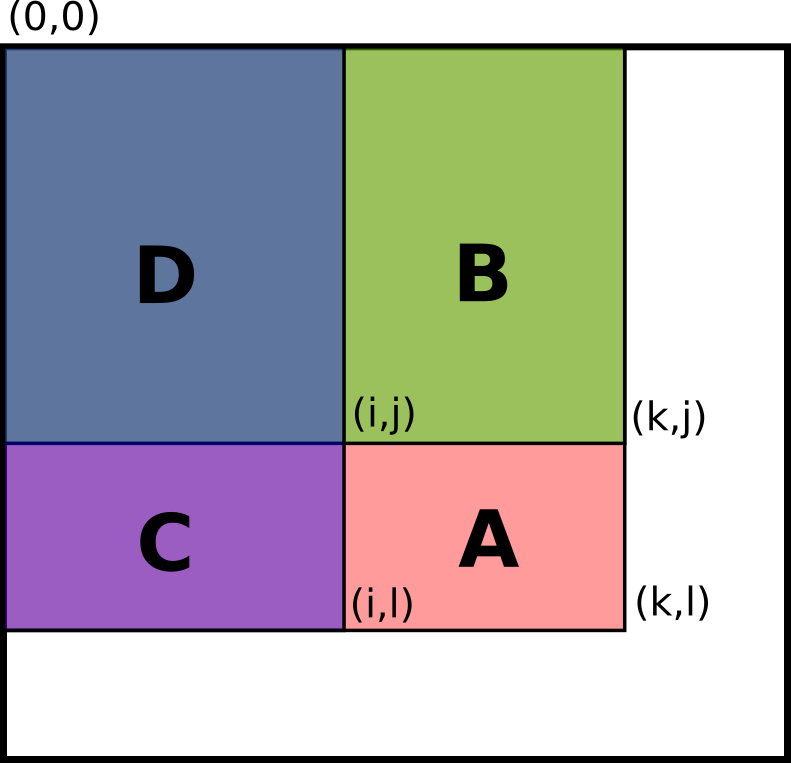
\includegraphics[width=\textwidth]{img/inclusion_exclusion}
  \column{0.5\textwidth}
  \[A = ABCD - BD - CD + D\]
\end{columns}

\end{frame}

\begin{frame}[fragile]{Maximum Range Sum 2D}{2D Sum Table Pseudocode}
\begin{block}{}
{\smaller
\begin{verbatim}
for i in (0:n):                      // Creating the Sum Table
   for j in (0:n):
       ST[i][j] = A[i][j]            // A[i][j] is the input
       if (i > 0) ST[i][j] += ST[i-1][j]
       if (j > 0) ST[i][j] += ST[i][j-1]
                                     // Avoid double count
       if (i > 0 && j > 0) ST[i][j] -= ST[i-1][j-1]

for i,j in (0:n)(0:n):
   for k,l in (i:n)(j:n):
      sum = ST[k][l]                 // Total Sum (0,0)->(k,l)
      if (i > 0) sum -= ST[i-1][l];  // Remove (0,0)->(i-1,l)
      if (j > 0) sum -= ST[k][j-1];  // Remove (0,0)->(k,j-1)
      if (i > 0 && j > 0) sum += A[i-1][j-1]
                                     // Add back double remove
      maxsum = max(sum,maxsum)
\end{verbatim}
}
\end{block}

\end{frame}

\subsection{Longest Increasing Subsequence}

\begin{frame}[fragile]{Problem 3: Longest Increasing Subsequence}{Problem Definition}
  \begin{block}{}
    Given a sequence $A$ of integers, find the longest subsequence $S \in A$ where $S_i < S_{i+1} < S_{i+2} < \ldots$.
  \end{block}
  \bigskip

  Example:
\begin{verbatim}
A   = [-7, 10, 9, 2, 3, 8, 8, 1]
S_1 = [-7,        2, 3, 8]          // size 4 -- LIS
S_2 = [-7,     9]                   // size 2
\end{verbatim}
\bigskip

Note that because the subsequence is {\bf not contiguous}, this problem is more difficult than Range Sum.
\bigskip

{\bf QUIZ}: What is the \alert{Complete Search} and \alert{DP approach} (Table and Transition) for this problem?
\end{frame}

\begin{frame}[fragile]
  \frametitle{Complete Search for LIS}

  As other "find the subset" problems, the complete search of LIS can be done by testing all binary strings of size "n". This costs $O(2^n)$.
  \smallskip

  \begin{block}{}
    {\smaller
\begin{verbatim}
// Complete Subset Search using bitmasks
vector<int> S_max; int max_len = 0;// Final Result

for (int i = 0; i < (1<<n); i++) { // Loop all bitstrings
  vector<int> S;
  int min = -99999; int len = 0;
  for (int j = 0; j < n; j++) {  // Creat subset from bitstring
    if ((1<<j)&i) {              // Add j to subset
      if (A[j] > min) {          // Test if subset is increasing
        S.push_back(A[j]);
        min = A[j]; len ++;
      } else { break; }          // Subset not increasing
  } }
  if (len > max_len) {           // Found a longer subset
    max_len = len; S_max = S;
} }
\end{verbatim}
    }
  \end{block}
\end{frame}

\begin{frame}{DP for Longest Increasing Subsequence}
  As usual, to prepare a DP we decide the {\bf Table} and {\bf Transition}.

  \begin{block}{Transition}
    For every element A[i], that element is either:
    \begin{itemize}
      \item The beginning of a new partial LIS;
      \item Added to the end of an existing partial LIS;
    \end{itemize}
    So for each element, we only need to know which partial LIS this item should be added to.
  \end{block}

  \begin{exampleblock}{Table}
    \begin{itemize}
      \item {\bf Parent}: Indicate the previous element of the longest partial LIS this element is a member of;
      \item {\bf LIS}: Indicate the current size of the longest partial LIS this element is a member of;
    \end{itemize}
  \end{exampleblock}
\end{frame}

\begin{frame}[fragile]{DP for Longest Increasing Subsequence}{Example}
\begin{verbatim}
  A      = [ -7, 10, 9, 2, 3, 8, 8, 1 ]
  parent = [ -1,  0, 0, 0, 3, 4, 4, 0 ]
  LIS    = [  1,  2, 2, 2, 3, 4, 4, 2 ]
\end{verbatim}

\begin{block}{Pseudocode (O($n^2$))}
\begin{verbatim}
LIS[0:n] = 1
parent[0:n] = -1
for i in (1 to n):
   for j in (0 to i): // Try to add to longest LIS
      if (LIS[j] >= LIS[i]) && (A[j] < A[i]):
         LIS[i] = LIS[j] + 1
         parent[i] = j
\end{verbatim}
\end{block}

There is a faster $O(n\log k)$ approach that uses greedy and binary search. I'll leave that one for you to find by yourself!
\end{frame}


\subsection{Knapsack problem}
\begin{frame}[fragile]{Classic DP: The 0-1 Knapsack Problem}

  In the 0-1 Knapsack problem (also known as "subset sum"), there is a set $A$ of items with size $S$ and value $V$.\bigskip

  You have to select a subset $X$ where the sum of sizes is under $M$, and the sum of values is as high as possible.\bigskip

\begin{verbatim}
Input:
  A<S,V> = [ (10, 100), (4, 70), (6, 50), (12, 10)]
  M = 12

Solution:
  [ (4,70), (6,50) ]
\end{verbatim}\bigskip

{\bf QUIZ}: What is the complete search and the DP (Table, Transition)?\\
{\bf Hint:} This problem is similar to the "Wedding Problem".
\end{frame}

\begin{frame}[fragile]{0-1 Knapsack -- Complete Search}
  The solution to the complete search is to test all subsets of A. This approach, as you know, takes $O(2^n)$.\bigskip

  This time, instead of a binary string, we will test all combinations using {\bf recursion}.

  \begin{block}{Complete Search Recursive Solution}
    Recursive function: \emph{value(id,size)}, where \emph{id} is the item we want to add, and \emph{size} is the size remaining after we add id in the backpack.\medskip

\begin{verbatim}
value(id,size):
   if (size < 0): return 0   # bag is full
   if (id == n):  return 0   # checked all items
   # either add the item, or do not add the item
   return max(value(id+1,size),
              V[id] + value(id+1, size - S[id]))
\end{verbatim}
  \end{block}
\end{frame}

\begin{frame}[fragile]{0-1 Knapsack -- Top-down DP}
  Because we already have a recursive function, it is very easy to modify \emph{value(id,size)} to use a DP table as memory. Let's see an example:

\begin{verbatim}
A<S,V> = [ (10, 100), (4, 70), (6, 50), (12, 10)]
M = 12

value(i,size):
\end{verbatim}

  \begin{center}
  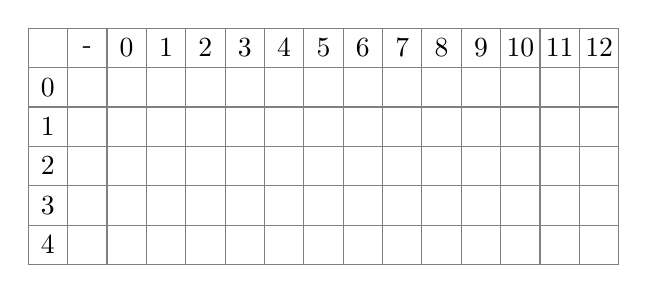
\begin{tikzpicture}
  \draw[step=0.5cm,color=gray] (0,0) grid (7.5,3);
  %% Row 0
  \node at (.75,2.75) {-};
  \node at (1.25,2.75) {0};
  \node at (1.75,2.75) {1};
  \node at (2.25,2.75) {2};
  \node at (2.75,2.75) {3};
  \node at (3.25,2.75) {4};
  \node at (3.75,2.75) {5};
  \node at (4.25,2.75) {6};
  \node at (4.75,2.75) {7};
  \node at (5.25,2.75) {8};
  \node at (5.75,2.75) {9};
  \node at (6.25,2.75) {10};
  \node at (6.75,2.75) {11};
  \node at (7.25,2.75) {12};
  %% Column 0
  \node at (.25,2.25) {0};
  \node at (.25,1.75) {1};
  \node at (.25,1.25) {2};
  \node at (.25,.75) {3};
  \node at (.25,.25) {4};
  \end{tikzpicture}\bigskip
  \end{center}

  {\bf Be careful}: The DP table size (and the execution time) is $|A|\times M$. If $M$ is too big ($>> 10^6$), you might get TLE or MLE.
\end{frame}

\subsection{Coin Change}
\begin{frame}[fragile]{Classical DP -- The Coin Change Problem (CC)}{Problem Summary}
  You are given a target value $V$, and a set $A$ of coin sizes. You have to find the smallest sequence of coins (with repetition) that adds to $V$.
  \bigskip

Example:
\begin{verbatim}
V = 7
A = {1, 3, 4, 5}
  S_0 = { 1, 1, 1, 1, 3}
  S_1 = { 5, 1, 1}
  S_2 = { 3, 3, 1}
  S_3 = { 4, 3}
\end{verbatim}

The best solution is $S_3$.\bigskip

{\bf QUIZ}:
\begin{itemize}
  \item How do you solve this by complete search?
  \item What is the DP Table and Transition?
\end{itemize}
\end{frame}

\begin{frame}[fragile]
  \frametitle{Complete Search for Coin Change}

  We can build a recursive search using the following recurrence on the number of coins $N$ necessary for a given value $V$:
  \[N(V) = 1 + N(V-\text{ size of coin})\]

  \begin{block}{Recursive Complete Search}
    {\smaller
\begin{verbatim}
coins(V):                    // Number of coins for value V:
   if V == 0: return 0       // 0 coins for value 0
   if V < 0:  return MAX_INT // Can't satisfy for this value
   min = INF                 // Minimum number of coins
   for i in (coins):         // Test each coin
      t = 1 + change(value - A[i])
      if (t < min): min = t
   return t
\end{verbatim}
  }
  \end{block}
\end{frame}

\begin{frame}[fragile]{DP for Coin Change}
  \begin{itemize}
    \item Implementing a Top-down DP should be easy for you now;
    \item Let's make a Bottom-UP DP for practice.
    \item For Bottom-UP DP, it is easier to use a table indexed on COINS
  \end{itemize}

\begin{block}{Bottom-UP DP}
  {\smaller
\begin{verbatim}
boolean DP[c][v] = FALSE;     // Can we reach v with c coins?

i = 0; DP[0][0] = TRUE;       // Start condition
while (TRUE):
  i+=1; possible = FALSE      // Start the loop
  for j = 0 to V:
    if (DP[i-1][j]):          // For each reachable value of V
      possible = TRUE         // We can continue
      if (j == V): return c-1 // Found a solution, go back!
      for k in (coins):       // update all coins
        DP[i][j+k] = TRUE     // Mark new reachable values
  if (!possible): return -1   // No solution found
\end{verbatim}}
\end{block}
\end{frame}

\begin{frame}[fragile]{DP for Coin Change}{Simulation}
\begin{verbatim}
V = 7
A = {1, 3, 4, 5}
\end{verbatim}

\begin{center}
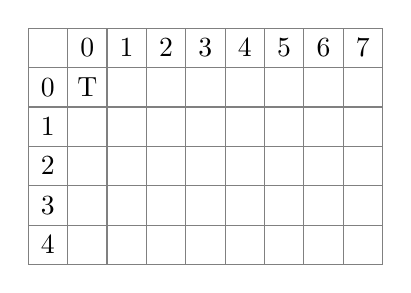
\begin{tikzpicture}
\draw[step=0.5cm,color=gray] (0,0) grid (4.5,3);
%% Row 0
\node at (.75,2.75) {0};
\node at (1.25,2.75) {1};
\node at (1.75,2.75) {2};
\node at (2.25,2.75) {3};
\node at (2.75,2.75) {4};
\node at (3.25,2.75) {5};
\node at (3.75,2.75) {6};
\node at (4.25,2.75) {7};
%% Column 0
\node at (.25,2.25) {0};
\node at (.25,1.75) {1};
\node at (.25,1.25) {2};
\node at (.25,.75) {3};
\node at (.25,.25) {4};
%% Starting Value
\node at (.75,2.25) {T};
\end{tikzpicture}\bigskip
\end{center}
\bigskip

It is interesting to note that the calculation of row $i$ depends only on row $i-1$. Using this information, you can implement the program with a much smaller table.

\end{frame}

%\subsection{Travelling Salesman Problem}
%\begin{frame}
%  \frametitle{Classical DP -- Travelling Salesman Problem}
%
%  We will talk about TSP with DP Next Class!
%\end{frame}

%%%%%%%%%%%%%%%%%%%%%%%%%%%%%%%
% Travelling Salesman Problem (bitmask again)
%% Travelling Salesman Problem (TSP)
% State: tsp(pos,bitmask)
% Transition:
%   Each visited city is a bit in the bitmask
%   - if every city has been visited: tsp(pos, 2^n -1) = dist[pos][0] (back to the start with 0 cities)
%   - Else, try visiting unvisited cities one by one
%   - tsp(pos,bitmask) = min (dist[pos][nxt] + tsp(nxt,bitmask|1<<nt))) for every nxt != pos,
%                                                                           and nxt not visited
%                                                                           bitmask & 1<<nxt == 0
